\documentclass[a4paper,10pt]{article}
\usepackage[a4paper, hmargin={1.5cm,1.5cm}, vmargin={1.5cm,1.5cm}]{geometry}
\usepackage{amsmath}
\usepackage{amssymb}
\usepackage{amsthm}
\usepackage{amsfonts}
\usepackage{color}
\usepackage{graphicx}

\title{Report Topics in Computational Science}
\author{Afifah Maya Iknaningrum \\ 1715011053}

\begin{document}
	\maketitle
	
%	\textbf{Problem : } For $ \alpha \in \mathbb{R}^+ $ and $ x(t) : \mathbb{R}^+ \rightarrow \mathbb{R} $, solve
%	\[ \dfrac{dx}{dt} = \alpha(1-x)x \]
%	Solution : $ x = \dfrac{1}{1+Ae^{-\alpha t}} $ where $ A = \dfrac{1-x(0)}{x(0)} $ \\ \\ \\
%	
%	\textbf{Answer : }
%	\begin{eqnarray} \nonumber
%	& \dfrac{dx}{dt} = \alpha (1-x) x \\ \nonumber
%	\Leftrightarrow & \dfrac{dx}{(1-x)x} = \alpha \ dt \\ \nonumber
%	\Leftrightarrow & \Big( \dfrac{1}{1-x} + \dfrac{1}{x} \Big) dx = \alpha \ dt \\ \nonumber
%	\Leftrightarrow & \int \dfrac{1}{1-x} \ dx + \int \dfrac{1}{x} \ dx = \int  \alpha \ dt & \text{(integrate both side) } \\ \nonumber
%	\Leftrightarrow & -\ln(1-x) + ln(x) = \alpha t + c & \text{(for any constant c )}\\ \nonumber
%	\Leftrightarrow & e^{-\ln(1-x) + ln(x)} = e^{\alpha t + c} & \text{(power by eksponential) } \\ \nonumber
%	\Leftrightarrow & e^{-\ln(1-x)} e^{ln(x)} = e^{\alpha t + c} \\ \nonumber
%	\Leftrightarrow & \dfrac{x}{1-x} = C e^{\alpha t} & \text{(for any constant $ C = e^{c} $ )}\\ \nonumber
%	\Leftrightarrow & \dfrac{1-x}{x} = A e^{-\alpha t} & \text{(for any constant $ A = 1/C $ )}\\ \nonumber
%	\Leftrightarrow & \dfrac{1}{x} - 1 = A e^{-\alpha t} \\ \nonumber
%	\Leftrightarrow & \dfrac{1}{x} = 1+A e^{-\alpha t}\\ \nonumber
%	\Leftrightarrow & x = \dfrac{1}{1+A e^{-\alpha t}}
%	\end{eqnarray}
%	For $ t=0 $ we obtain value of constant $ A $
%	\[ x(0) = \dfrac{1}{1+A} \Leftrightarrow A = \dfrac{1-x(0)}{x(0)} \]
%	such that the solution of the problem is
%	\[ x = \dfrac{1}{1+A e^{-\alpha t}} \]
%	where
%	\[ A = \dfrac{1-x(0)}{x(0) }\]	

Plot the solution of the following map
\begin{eqnarray}\nonumber
x_{n+1} &=& ax_{n}(1-x_{n}) \\ \nonumber
x_{0} &=& 0.35 \\ \nonumber
n  &=& 1,\dots,100
\end{eqnarray}
with
\begin{enumerate}
	\item $ a=0.5 $
	\item $ a=1.5 $
	\item $ a=3.3 $
	\item $ a=4.0 $
\end{enumerate}

\newpage
The sensitivity plot
\begin{figure}[h!]
	\centering
	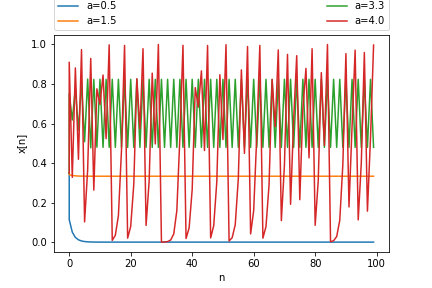
\includegraphics[width=0.7\linewidth]{sensitivity}
	\caption{Sensitivity}
	\label{fig:sensitivity}
\end{figure}

and the logistic map
\begin{figure}[h!]
	\centering
	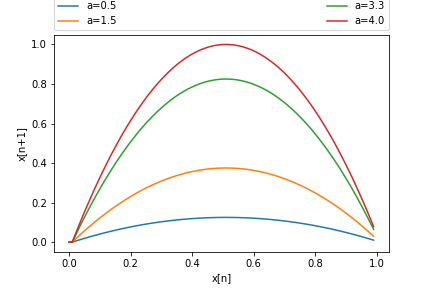
\includegraphics[width=0.7\linewidth]{logistic}
	\caption{Logistic}
	\label{fig:logistic}
\end{figure}



\end{document}